\section{Simulation System Engineering}\label{methodology-software}

\subsection{Requirements}

Based on the results and findings of the experiments presented in section \ref{methodology-basic}, we have come with a set of requirements for the next iteration of our simulation system.

It was decided to drop the older IveTrainer software in favour of developing a new system from ground up. IveTrainer was aimed to be a well scalable and extendable simulation system, but during the development many of the features were constructed in a poorly extendable way.

The updated software needs to adopt industry standard software design techniques. The software developed during this project also adheres to the `good' programming practices. Improved modularity and high coherence leads to unconstrained testing and functionality extension.

The new version of the system is required to be much more scalable and portable. The system is also required to include support for more sophisticated physical models.

\subsection{BirthEngine with .NET/Mono}

The .NET framework for the first iteration of reimplementing the simulation software. The new version of the software was named \textit{BirthEngine}.

\subsubsection{Crossplatform runtime}
  The Mono Framework \citep{mono_framework} is a cross-platform implementation of Microsoft's .Net framework that allows building and deploying .Net applications on platforms other than Microsoft Windows. By utilizing the framework the BirthEngine simulation system is capable of being run on multiple platforms.

The cross-platform capability of the framework come mainly from the fact that it has an intermediate run-time. As seen in Figure \ref{software-dotnet-runtime} the source code is compiled into another form that is then interpreted by the run-time of the target platform.

  \begin{figure}
  \begin{center}
  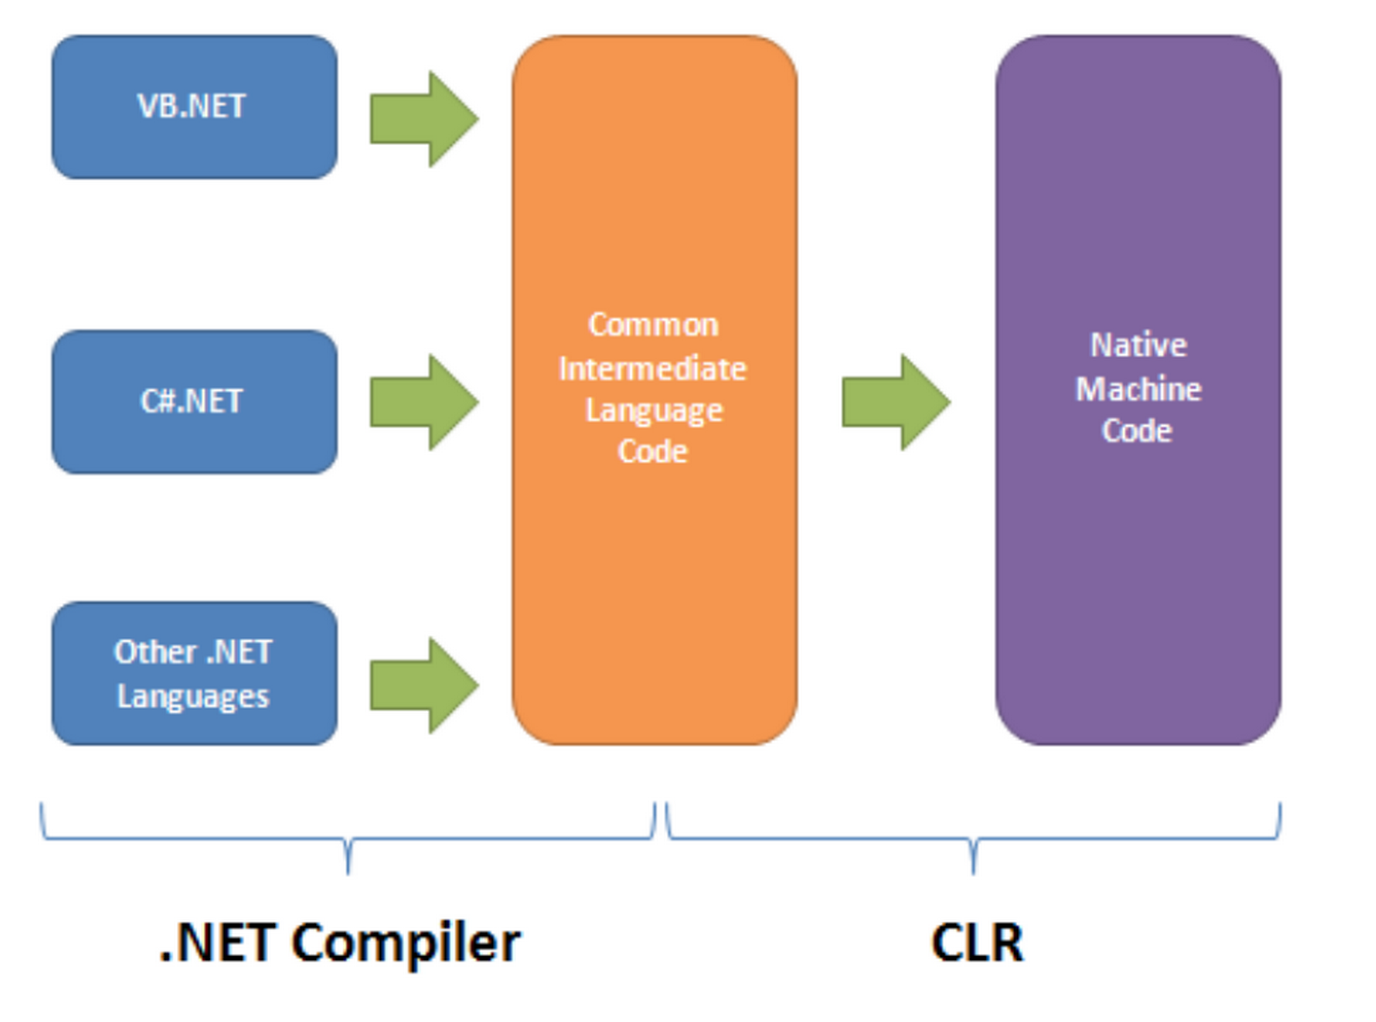
\includegraphics[width=80mm]{sections/methodology/images/software/dotnet-runtime.png}
  \caption[Entity component system use in BirthEngine.]{\label{software-dotnet-runtime} Entity component system use in BirthEngine.}
  \end{center}
  \end{figure}

\subsubsection{Rendering capabilities}

  Simulation systems often lack the appealing rendering capability of the more graphics oriented applications, such as games. However, we believe that having a realistic graphical representation of the simulation environment carries a great role in immersiveness of the scene, which in turn affects how effective the training is. Therefore, a considerable attention is given the graphical engine of the simulations sytem.

  OpenTK \citep{opentk} is an open-source toolkit that wraps around a number of low level API's. It provides access to the OpenGL, OpenAL and OpenCL API's of the target platform. OpenTK was used in developing the graphical component of the simulation system.

  The IveTrainer rendering engine was based on the less efficient OpenGL 2.0 API. The OpenGL 3.0 is used. The choise of using the third version of the API instead of the latest OpenGL 4.0 is justified by the requirement of backwards capability. The simulation system is inteded to work even on a less modern hardware, which will not necessarily support the latest OpenGL API.

  The chosen API is sufficiently modern to allow more realistic and efficient rendering capabilities. The list of advanced rendering techniques avaiable in software are list here:

  \begin{itemize}
    \item Shaders based rendering for a highly customizable rendering capabilities
    \item Deferred shading for efficient multi-light scenes
    \item Volumetric rendering of voxel data using ray-tracing in shaders
    \item Vertex Buffer Object based mesh rendering to minimize memory transfer times for increased rendering speeds
  \end{itemize}

  The rendering engine of BirthEngine is build around the low level API to allow easier and faster creation of graphical representation of simulations. Object-oriented abstractions are built on top of the C API.

\subsubsection{Limitations}

BirthEngine software is a generic, functional and extendable simulation system. It has been used by a Master student for his dissertation and performed very well in being a generic foundation for his simulation. The language and tooling kit simplify and improve productivity making it possible to develop large amounts functionality in short periods of time.

However, due to the nature of .NET and Mono run-times, as seen in Figure \ref{software-dotnet-runtime}, the performance of the application degrades quickly with increased computational loads. Particularly, collision detection, which involves a large amount floating point numerical calculations, slows down considerably with increased mesh sizes. We have not performed detailed benchmarkings, however we observed that the difference between a native C++ version \ref{birthview} can reach 2x timesteps.

\subsection{BirthView with C++/SDL2} \label{birthview}

The disadvantages of the BirthEngine simulation system required the next iteration of development be based on lower level \textit{native} techonologies. A run-time that has no overhead of an intermediate virtual machine needs to be used.

The next version of our simulation system was named BirthView and was based on low-level C++ language and API's. Precompiled and highly optimized C++ applications perform the best as compared to any other language.

\subsubsection{SDL}

The Simple DirectMedia Layer (SDL) is a cross-platform graphical application development library \cite{libsdl}. It provides access to low level API's of the underlying operating system in a platform-agnostic way. The same code-base can be used for deployng the application on Windows, Linux, Mac, Android and Ios.

The choise of SDL over other alternatives was mainly due to the fact that it has a wider cross-platform support. Additionally, it is possible to deploy onto mobile devices. In a distant future it is possible that certain aspects of our simulation software maybe ported onto mobile devices.

\subsubsection{Modular architecture}

BirthView was built with modularity and scalability in mind. The main approach towards a madular structure is plugin based extendability. The additional functionality of the system, which is not its generic core part, is contained in a separate project. As seen in Figure \ref{software-birthview-projects} the BirthView solution contains several projects each of which represent a plugin extending the generic simulation system.

\begin{figure}
\begin{center}
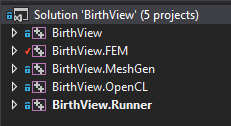
\includegraphics[width=80mm]{sections/methodology/images/software/birthview-projects.png}
\caption[BirthView solution's list of plugin projects.]{\label{software-birthview-projects} BirthView solution's list of plugin projects.}
\end{center}
\end{figure}

Currently there are three plugins for BirthView simulation system created:


\begin{description}
  \item[OpenCL] \hfill \\
  Contains all of the functionality related to specializing BirthView to use OpenCL for parallel processing. Can be easily replaced by an equivalent plugin bringing in support for alternative parallelization API's like CUDA.
  \item[FEM] \hfill \\
  Contains all of the TLED FEA related routines and data-structures. The justification of separting this functionality into a separate plugin is due to the fact that not all simulations require FEA.
  \item[MeshGen] \hfill \\
  Contains the initial implementation of the intended FE mesh generation functionality. Currently contains rudimentary mesh generation routines.
\end{description}

The same modular architecture is implemented in BirthEngine as well.

\subsubsection{Entity Component System}

Entity component system (ECS) is a popular framework primarily used in high-performance oriented graphical applications development, particulary in game development. The framework is an example of a broader approach to software engineering known as \textit{Composition Over Inheritance}. The approach is a well known design pattern and can be found in the book \citep{Freeman:2004:HFD:1076324}.

ECS is chosen as the core approach to describing the simulation elements and their behaviours. The main idea is that each simulation object is represented by an \textit{entity}. Typically, all scene elements are entities directly and not through inheritance. However, in cases when certain behaviour is commonly present in many enities. Example of such a subclass is \textit{Model} that has the rendering capabilities built-in, as oposied to manually attaching components responsible for rendering.

The class diagram in Figure \ref{software-ecs} provides an example of how ECS is used to represent a part of a simulation scene. The entity representing the pelvic floor is a subclass of the \textit{Entity} class. It contains several \textit{Component} subclasses each specifying a particular behaviour. The behaviour of the entity can be easily modified by adding, removing or replacing the attached components. For example, removing \textit{RenderableComponent} instance will make the entity invisible. Simillarly, removing the Finite Element

Note that the pelvic floor entity does not not need to be a subclass, as it could simply be an instance of the \textit{Entity} class with an appropriate name and a collection of components.

\begin{figure}
\begin{center}
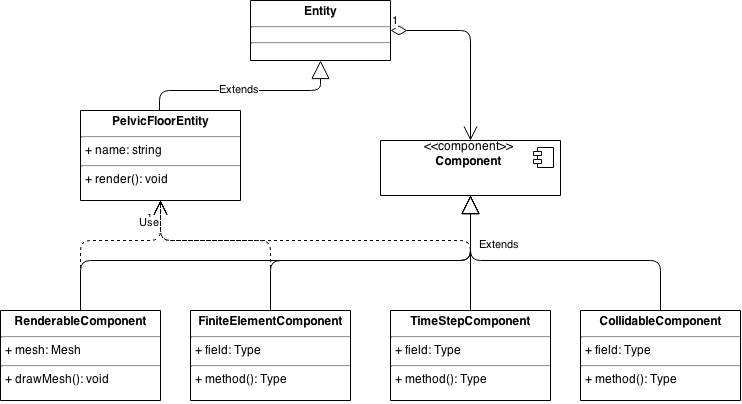
\includegraphics[width=110mm]{sections/methodology/images/software/software-ecs.png}
\caption[Entity component system use in BirthEngine.]{\label{software-ecs} Entity component system use in BirthEngine.}
\end{center}
\end{figure}
